\chapter{接口误用缺陷静态检测技术}
\label{cha:imchecker}
软件库通过应用编程接口(API)来封装已有功能,从而提高现代软件开发效率。
正确的接口使用需要满足特定的约束,否则将引入接口误用,导致接口误用缺陷。
静态检测技术是在不运行程序的前提下对程序行为进行分析的技术,
能够在开发早期进行应用,
极大地降低缺陷修复的成本。
现有的静态检测技术可以分为两类,基于程序分析的缺陷检测技术和基于数据挖掘的缺陷检测技术。
虽然现有工作能够对实际缺陷进行检测,但是随着现代软件规模扩大结构复杂以及开源代码的广泛使用,
现有工作面临检测精度与规模的矛盾关系。
一方面,现有工作支持的缺陷模式和目标接口固定难以扩展,对用户自定义的接口支持不足;
另一方面,语义分析不足,大规模程序检测结果不精确。
因此,研究精准高效的C程序接口误用缺陷检测技术,对于提升软件系统可靠性和安全性具有重要意义。

本章旨在研究规模化接口误用缺陷静态检测技术,以对大规模程序中多种接口误用缺陷进行准确、高效的检测,
弥补现有静态检测技术不足。
本章首先基于第\ref{cha:imchecker}章的缺陷模式对现有检测工具和方法进行分析,
总结现有工作的特点和不足。
接着提出基于约束描述的C程序规模化接口误用缺陷检测方法IMChecker。
IMChecker通过IMSpec语言对接口使用约束描述,从而支持多种缺陷模式和用户自定义的接口;
基于多入口分析策略以应对实际项目中大规模代码;并基于语义信息和统计信息对结果的精度进行提升。
从全文的研究体系上看,
本章的工作是描述语言IMSpec的应用,同时是接口误用缺陷检测实际应用的重要核心。

\section{引言}
开发者在利用API快速构建系统的同时,需要满足接口使用的约束条件,从而正确执行接口内部封装的功能。
否则,将会产生接口误用导致软件缺陷。
对接口误用检测技术研究具有重要意义。
一方面,接口误用是导致软件错误、系统崩溃、漏洞产生的重要原因之一。
CWE组织2011年发布的最危险25种软件错误中,有40\%和接口误用相关~\cite{cwe-top25}。
同时,OWASP项目在2017年发布的最危险10类网络漏洞中,有30\%和接口误用相关~\cite{owasp-top10}。
另一方面,随着开源社区的发展,软件库文档缺失、开发人员对API理解不足,
导致现有的代码中存在大量的接口误用缺陷。

近年来,研究人员设计并实现各种各样的方法来检测接口误用缺陷。
特别地,静态检测技术获得广泛的关注和应用。
静态检测技术能够在不执行代码的情况下进行分析,
可以应用于开发的各个阶段,有效地提高代码质量。
同时,静态分析在使用时可以不借助人工标记、构造测试用例和测试环境搭建,
因此能够对所有的程序路径进行模拟执行使用范围广。
针对于接口缺陷检测,从分析策略上来说静态分析包含两种主要的技术路线:
程序分析技术~\cite{16-saner-evaluation}和数据挖掘技术~\cite{survey18}。
基于程序分析技术的检测方法和工具需要研究人员和工具实现者具备接口使用的领域知识,
通过规约描述或者程序硬编码的方式对目标接口使用的约束进行预先定义。
此后,基于程序语义通过可达性分析、程序语义匹配等方式进行缺陷检测。
基于数据挖掘技术的方法和工具则通过统计学习的方法,
根据算法设计者预定义的模式在项目中进行接口使用约束推理。
此后,基于推理的约束从统计意义角度进行缺陷检测。

虽然两者都能够在实际项目中进行应用并找到新的接口误用缺陷,
然而在现代软件开发模式下,两者存在两个主要不足:
(1)缺陷模式难以扩展,对用户自定义的接口支持不足。
前者无法应用于未定义的目标API,后者则依赖于大量高质量的数据从而学习正确的接口使用约束条件。
(2)语义分析不足,分析精度不够,难以应用于实际项目中。
一方面,现有的工具多基于语法层分析;另一方面,为支持大规模代码,
工具多在过程内分析忽略过程间的语义信息。


为解决上述方法中的不足,平衡分析精度与规模的矛盾关系,
本章提出基于约束描述的规模化接口误用缺陷静态检测方法IMChecker。
首先,IMChecker通过IMSpec规约描述以支持多种缺陷模式和用户自定义的接口。
精度和效率是静态分析技术需要平衡的重要指标。
高精度的分析技术需要昂贵的计算代价,从而限制静态分析在实际项目上应用效果。
高效率的分析技术则存在分析精度的损失,产生大量的误报(False Positive, 将正确行为报告为缺陷)
和漏报(False Negative,实际缺陷没有被检测出)。
因此,IMChecker基于多入口分析策略,将复杂的程序分析问题分而治之,
高效率分析的同时实现局部的精确分析。
针对多入口分析策略导致的分析精度损失,
IMChecker通过基于上下文的语义摘要信息和基于使用情况的统计信息进行结果过滤,
以提高检测的精度。
本章基于开源缺陷测试集Juliet Test Suite中13个接口缺陷相关的CWE分类对IMChecker方法进行评估。
实验结果显示,IMChecker方法误报率为13.21\%,漏报率为16.08\%。
检测能力领先于主流的开源检测工具。

本章其余部分组织结构如下:
\ref{sec:3.2}节对相关研究进行总结,
\ref{sec:3.3}节对规模化接口误用缺陷静态检测算法进行介绍,
\ref{sec:3.4}节给出工具实现和评估结果,
最后在\ref{sec:3.5}节总结本章工作。
\section{相关工作}
\label{sec:3.2}

静态缺陷检测方法在不执行程序的情况下,对程序中的缺陷进行检测。
针对C程序接口误用缺陷,
近年来研究人员和工具开发者设计并实现各种各样的静态检测算法和工具~\cite{16-saner-evaluation, survey18}。
本节对其中的典型算法和工具进行调研和总结。
从技术路线上来说,静态缺陷检测方法可以分为两大类,
\begin{itemize}
	\item {\kaishu 程序分析技术}
	程序分析技术需要显式地提供目标接口的使用约束,
	因此需要研究人员和开发者具有良好的领域知识。
	目前,约束的描述方式有两种:规约描述语言和程序硬编码检测插件。
	前者在分析的过程中,首先将语言进行解析并构造监控自动机的中间表达或进行代码插桩。
	在程序语义分析阶段,通过可达性分析、程序属性图搜索、语义匹配等方式缺陷进行检测。
	基于描述的方法有利于对新的接口进行扩展,即提供对应的缺陷描述。
	后者则在分析的过程中,利用预先实现的检测插件进行缺陷检测,
	因此该方法难以扩展,即需要实现新的检测器。
	基于程序分析技术的工作,最大的优点是可以有效利用积累的领域知识,并利用语义分析获得更加准确的分析结果。
	\item {\kaishu 数据挖掘技术}
	数据挖掘技术则不需要用户提供显式的约束,
	可以基于统计信息通过学习的方法自动推理约束。
	其检测的核心在于,通过对程序形式的转化构造中间表达,
	并基于预先定义的模式学习接口使用的约束。
	特别地,大多数方法认为:多数使用为正确用法,少数则为错误。
	虽然基于数据挖掘技术的检测方法不需要人工定义具体的约束,
	但是需要良好领域知识设计学习模型。
	因此,其扩展性有限。
	基于数据挖掘技术的工作,最大的优点是设计好学习模型后可以实现完全自动化,同时可以应用于不同项目。
\end{itemize}

如表\ref{tab:3-2-survey}中所示,本文共对17个研究工作和工具进行调研和总结。
其中前五个为基于程序分析技术的普适性静态缺陷检测工具,包括三个开源软件(Clang-SA、Cppcheck和Infer)
以及两个商业工具的学术使用版(Pinpoint和Coverity)。
第6-7个为面向接口使用领域基于程序分析技术的静态缺陷检测工具。
最后10个则为基于数据挖掘技术的程序接口缺陷检测技术和工具。
针对提供实际工具的工作,本文对工具进行使用;
对于没有工具的工作,本文对论文进行阅读,总结其检测能力。
特别地,为减少本文主观臆断带来的影响,
对于每一个工作本文或直接与论文作者进行结果核对;
或同时阅读3-5个引用该论文的其他工作,与这些论文中的描述进行核对。

\begin{table}[t]
	\centering
	\begin{minipage}[t]{0.85\linewidth} % 如果想在表格中使用脚注,minipage是个不错的办法
		\caption{静态分析工具对C程序接口缺陷检测能力}
		\label{tab:3-2-survey}
			\begin{tabular}{@{\extracolsep{3pt}}ccccccccccc@{}}
			%\begin{tabular}{ccccccccccc}
			\hline
			\multirow{2}{*}{工具名称} & \multicolumn{2}{c}{IPU\footnote{Y:支持,P:部分支持,-:不支持}} & \multicolumn{3}{c}{IEH} & \multicolumn{3}{c}{ICC} & \multirow{2}{*}{扩展性\footnote{难:难以扩展,有限:可以扩展,扩展内容受限,-:不支持,$\checkmark$:方便扩展}} & \multirow{2}{*}{可用性\footnote{$\checkmark$:可用且基本符合预期,P:可用但与预期相差很大,-:不可用}} \\
			\cline{2-3}\cline{4-6}\cline{7-9}
			 & -s & -r & -c & -p & -l & -s & -c & -r & & \\
			\hline
			Clang-SA~\cite{clang-sa} & Y & Y & - & - & - & Y & Y & Y & 难 & $\checkmark$ \\
			Cppcheck~\cite{cppcheck} & Y & Y & P & - & P & Y & Y & Y & 有限 & $\checkmark$ \\
			Infer~\cite{infer} & Y & Y & - & - & - & Y & Y & Y & - & $\checkmark$ \\
			Pinpoint~\cite{pinpoint} & Y & Y & P & - & - & Y & Y & Y & - & $\checkmark$ \\
			Coverity~\cite{coverity} & Y & Y & Y & P & P & Y & Y & Y & 难 & $\checkmark$ \\
			\hline 
			SLAM~\cite{slam} & Y & Y & Y & - & - & Y & Y & Y & 有限 & $\checkmark$ \\
			SSLINT~\cite{15-sp-sslint} & P & - & Y & - & - & Y & Y & - & 有限 & - \\
			\hline
			PR-Miner~\cite{05-fse-prminer} & - & - & - & - & - & Y & Y & - & - & - \\
			RGJ07~\cite{07-PLDI-RGJ07} & Y & Y & - & - & - & Y & Y & - & - & - \\
			Chronicler~\cite{07-icse-chronicler} & - & - & - & - & - & Y & P & - & - & - \\
			EDP~\cite{08-fast-eio} & - & - & Y & Y & - & - & - & - & - & - \\
			Hector~\cite{13-dsn-hector} & - & - & - & - & - & Y & P & - & - & - \\
			Chucky~\cite{13-ccs-chucky} & P & P & Y & - & - & - & - & P &  & \checkmark \\
			NDNR14~\cite{14-fse-pre} & P & Y & - & - & - & - & - & - & - & - \\
			APISan~\cite{16-sec-apisan} & P & P & Y & Y & - & Y & Y & P & - & \checkmark \\
			Antminer~\cite{16-icse-antminer}& P & P & Y & P & - & P & P & - & - & - \\
			ErrDoc~\cite{17-fse-errdoc}& - & - & Y & Y & P & P & - & - & 有限 & P \\
			\hline
		\end{tabular}
	\end{minipage}
\end{table}

本文从三个方面对目标研究工作和工具进行调研和总结,
即检测能力、扩展性和可用性。
如表\ref{tab:3-2-survey}中所示,第一列为项目名称。
第2-9列为工具对于第\ref{sec:2.3}节中总结的接口误用缺陷模式的支持情况。
特别地,IPU-s代表单个参数的检查、IPU-r代表参数之间和参数与返回值之间的检测;
IEH-c代表异常处理中对接口返回值的检测、IEH-p为异常处理中返回错误代码的检测(error propagation)、
IEH-l为异常处理中对缺陷信息打印支持的检查;
ICC-s为不带上下文关系的接口对、ICC-c为带有上下文关系的接口对、ICC-r代表重复调用的检测。
第10列扩展性关注算法和工具是否预留扩展的接口,能够针对用户需求对项目特定的接口检测进行扩展。
其中难表示可以扩展但是代价较大,比如Clang-SA需要重新设计检查器插件;
有限代表工具提供扩展的方式但是扩展的内容需要满足特定的缺陷模式。
最后一列为工具的可用性,即该工具是否可用。
特别地,工具的效果是否和发表的论文、工具说明一致。
其中,P代表工具可以下载和使用但是其功能和论文描述不符,
即工具难以支持论文中明确给出的代码样例。

检测能力方面,
从表中调研结果可知在所有的工作中并没有一个工作能够完全的支持所有的接口缺陷模式。
特别地,基于数据挖掘技术的工作中部分(40\%)工作只能处理某一类缺陷模式,
绝大部分(80\%)工作不能支持所有类别。
检测能力最好的是商业工具Coverity和基于数据挖掘技术的工具APISan。
然而前者实际价格昂贵,难以广泛使用。
后者基于数据挖掘技术,本文对工具试用时发现具有极高的误报率
(工具作者在论文和工具主页中同样指出高误报率)。
此外,在所有缺陷模式中,单个参数检查、异常处理中返回值检查和
不带有上下文语义关系的函数调用对检查被大多数工具支持。
这些缺陷模式相对简单,能够从语法结构直接进行检查。
然而,本文发现绝大部分工具并没有考虑足够的语义信息。
例如,对于参数的检查,如果缺少参数或者代码中参数与常量比较则工具支持效果较好;
但是如果比较的方式是变量比较,则工具存在大量漏报。

扩展性方面,只有6个工具提供扩展的接口。
其中Clang-SA和Coverity需要设计新的检测器插件,扩展难度极大。
SLAM、SSLINT和Errdoc可以通过撰写规约的方式对检测目标扩展,
然而其只能针对于特定的缺陷模式或者项目特定的接口扩展,
即SLAM针对于Windows操作系统内核的驱动程序设计、SSLINT针对于SSL/TLS安全协议设计和
Errdoc针对于异常处理设计。
Cppcheck为用户提供最方便的扩展方式,
通过提供结构化的接口使用描述方式,用户可以对自定义的接口进行扩展。
然而,Cppcheck提供的扩展语言只能够支持单个参数、参数关系、返回值检测和不带因果关系的函数对四种情况。

应用性方面,基于数据挖掘的工作中可用的工具只有Chucky和APISan。
Errdoc工具在试用时,本文发现其与论文描述差距较大。
基于程序分析技术的工具本文选择的都是可以使用的工具,因此实用性较好。
然而,在实际项目应用中本文发现这些工具的分析报告存在两种极端的表现,
即要么报告数量多但存在大量的误报;要么报告数极少,与其他工具相比存在大量的漏报。

总体来说,针对C程序接口误用缺陷检测,现有的工作存在两点主要不足:
(1)缺陷模式支持有限扩展性不足,难以支持用户自定义的接口。
一方面,基于程序分析的技术需要通过规约撰写或者开发新的检测插件。
如第\ref{sec:2.2}节和本章调研结果所示,现有的约束描述方法或过于复杂,
或难以扩展到全部接口缺陷模式。
同时,开发新的插件则需要理解工具框架和细节,难以实际使用。
另一方面,基于数据挖掘的技术需要大量可靠数据进行约束条件的学习。
然而,该需求对于独立的项目难以实现。
特别地,用户自定义的接口往往使用次数有限,
难以满足学习所需要的数据量。
(2)语义分析不足,检测结果存在大量误报和漏报,难以支持实际项目分析。
一方面,为提高缺陷检测的效率,现有的工具多基于语法结构进行缺陷分析。
因此,难以支持需要语义信息的缺陷类型。
另一方面,多数工具基于过程内分析策略,以应对大规模程序。
然而,丢失的上下文语义信息会导致误报和漏报。

\section{接口缺陷静态检测方法}
\label{sec:3.3}
本节提出IMChecker,基于约束描述的规模化接口误用缺陷检测方法,与上述工作形成互补。
首先,IMChecker利用IMSpec领域特定语言描述接口使用约束,
以支持常见约束类型和用户自定义的接口,扩展检测的应用范围。
接着基于多入口分析方法将复杂的程序分析问题分而治之,
以提供全局高效分析的同时实现局部的精确分析。
最后,通过上下文的语义摘要信息和使用情况的统计信息对检测结果过滤,以提高检测的精度。
下文中,本文将通过图\ref{fig:1-1-example}中不包含修复片段代码作为案例,
介绍IMChecker方法的流程和核心思想,并对其中的关键步骤进行详细解释和分析。

\begin{figure}[b]
	\centering
	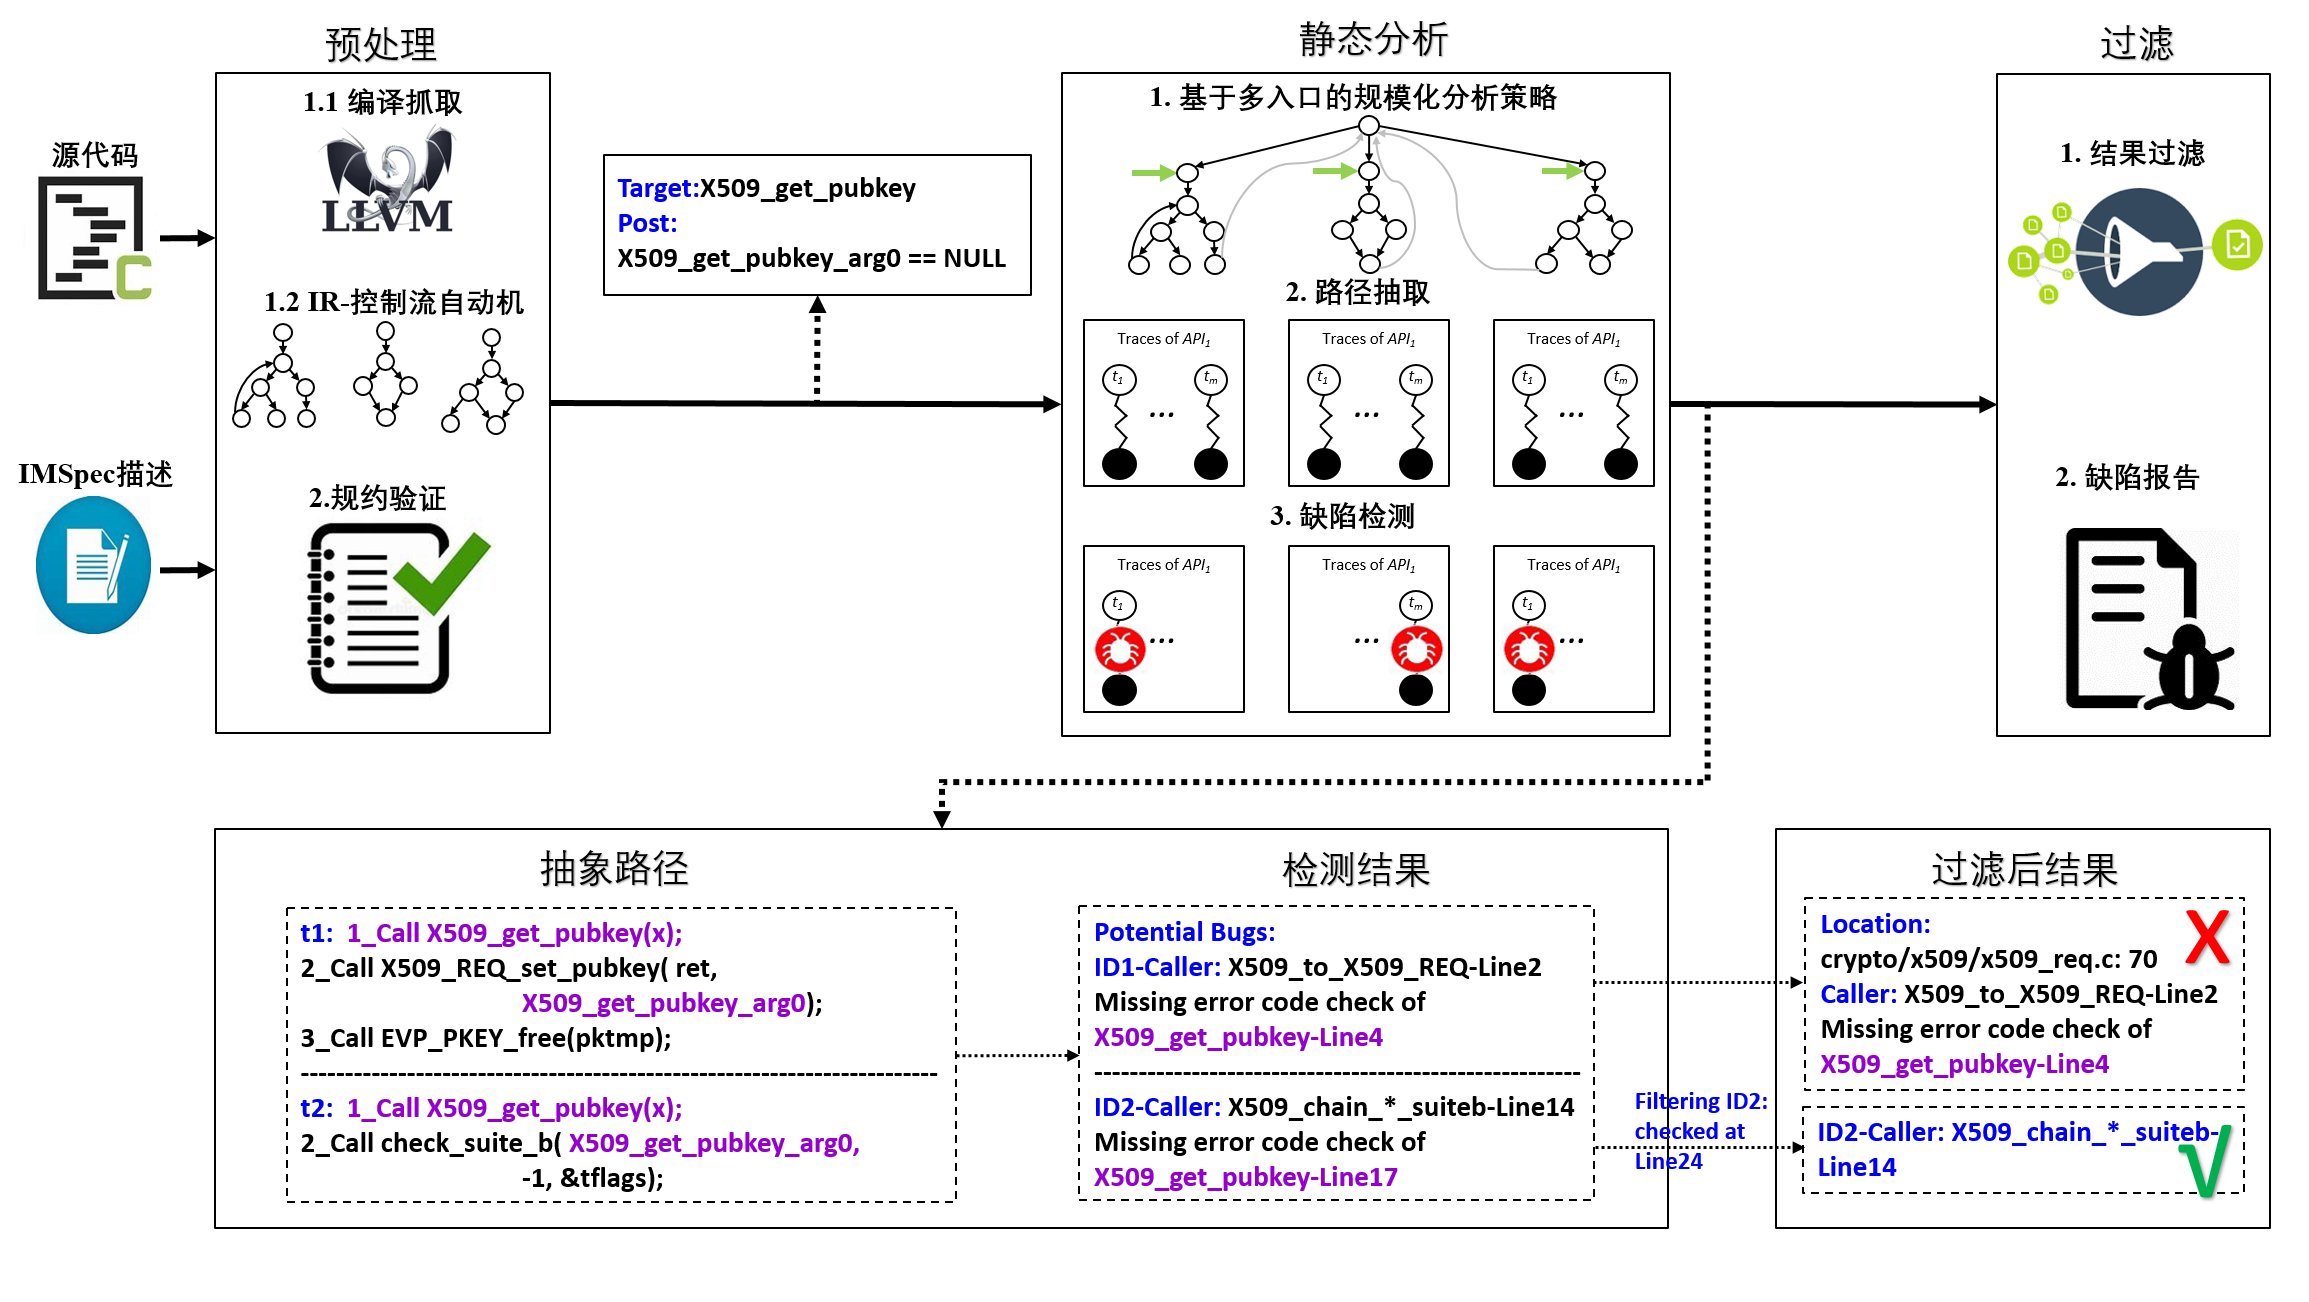
\includegraphics[width=\linewidth]{figures/cp3-3-overview.png}
	\caption{
		IMChecker工作流图
	}
	\label{fig:3-3-overview}
\end{figure}

\subsection{IMChecker工作流}

如图~\ref{fig:3-3-overview}中所示,IMChecker的工作流程包含三个主要步骤:
预处理、静态分析和过滤。

预处理阶段,IMChecker以用户提供的源代码和IMSpec描述文件作为输入,构造分析的上下文环境。
一方面,将源代码进行预处理,生成LLVM-IR\footnote{http://releases.llvm.org/3.9.1/docs/LangRef.html}中间表达。
并基于IR指令构造程序的控制流自动机(Control-Flow Automaton,CFA)。
另一方面,IMChecker解析IMSpec约束描述实例。
对接口使用约束进行划分,将一个目标接口的描述根据语义分解成调研中总结出的三大类约束模式,
确定缺陷检测的目标。

分析阶段,IMChecker首先根据CFA的结构,基于多入口分析策略选择入口,
以支持大规模程序分析。
针对每个待分析入口,根据接口使用的特点,基于符号执行技术在过程内抽取路径信息,
在保留有效语义的情况下简化程序结构。
接着利用接口误用缺陷检测算法,通过模式匹配的方式对目标接口的路径信息和使用约束进行检测,
并生成初步的检测结果。
例如,图\ref{fig:3-3-overview}中下侧给出图\ref{fig:1-1-example}中例子的抽象路径。
针对该用例,共存在两条不满足使用约束的路径。

过滤阶段,IMChecker利用上下文的语义信息和使用情况的统计信息对结果进行过滤与排序。
前者面向由于过程内路径提取和多入口分析策略带来的上下文信息丢失所导致的误报。
后者则针对于接口使用特殊用法或者IMSpec描述中的错误。
针对图\ref{fig:1-1-example}中例子,基于上下文的语义信息可知
第二条路径中缺失的非空指针约束在指针使用之前进行检查。
因此,第二条路径被过滤,从而最终的缺陷报告只有一个。

下文中,将对IMChecker方法中的关键步骤进行详细介绍。

\subsection{构造分析上下文}
基于静态分析的缺陷检测技术需要对纯文字的C程序源代码进行预处理,构造中间表达。
目前常用的方式有字节流(Token)、抽象语法树(Abstract Syntax Tree)、
自定义的的中间表达(intermediate representation)等等。
同时,基于这些中间表达构造图模型,将缺陷检测问题转化为图遍历问题或者图的可达性问题等等。
IMChecker采用LLVM-IR作为中间表达,
并基于CFA创建图模型,
构造分析上下文。

IMChecker对用户提供的源代码通过预编译的方式生成LLVM-IR中间表达。
LLVM-IR旨在提供一个轻量级、低级别、高表达能力的程序语义表示形式,支持类型信息且易扩展。
它的目标是成为一种“通用IR”,
通过低层次的语义表达将高层次的语言完全地映射到LLVM-IR。
即类似于微处理器的IR方式,允许许多源语言进行映射。
通过提供类型信息,LLVM-IR可以用于各种程序分析任务中。
LLVM-IR具有静态单侧赋值的属性(SSA),并且每个指令具有原子语义。
因此,可以将复杂的C语句转化为一系列的原子操作,方便语义的计算。

\begin{figure}[t]
	\centering
	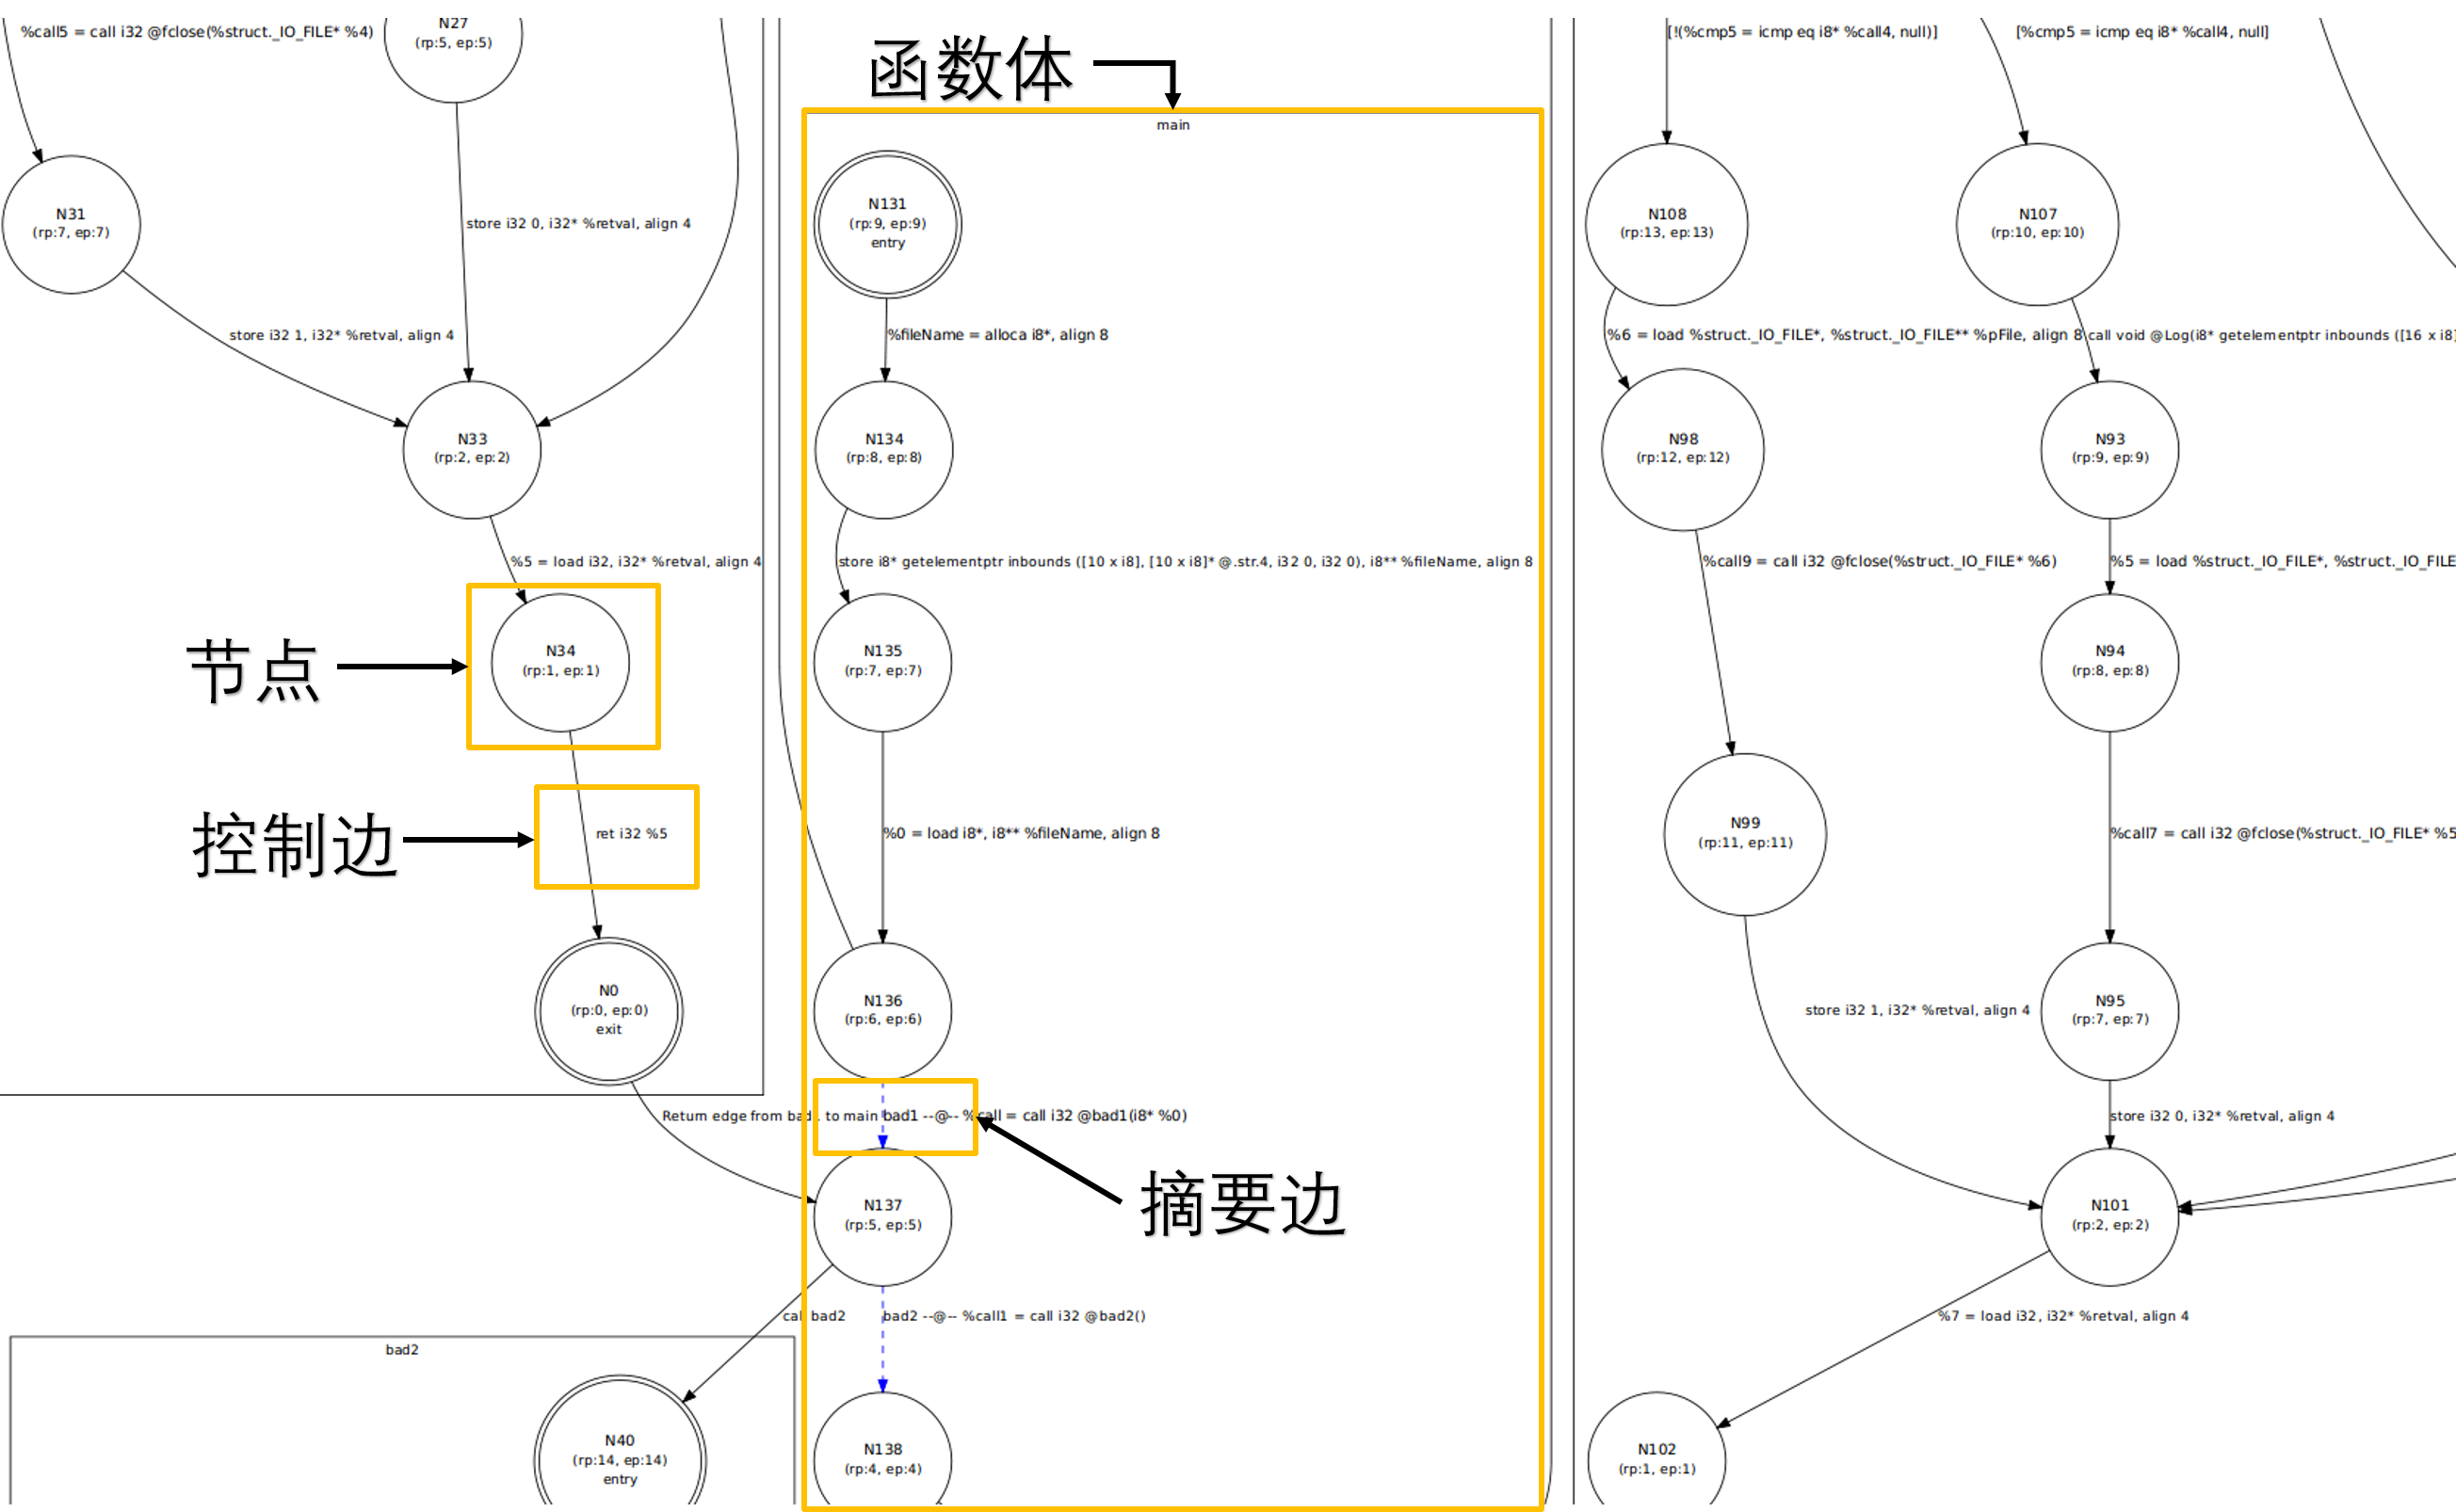
\includegraphics[width=0.7\linewidth]{figures/cp3-3-cfa.png}
	\caption{
		CFA示意图
	}
	\label{fig:3-3-cfa}
\end{figure}

在预处理生成LLVM-IR后,IMChecker基于CFA构造程序图结构。
如图\ref{fig:3-3-cfa}中所示,CFA以指令位置$l \in L$为节点,
以控制流操作的指令$e \in E = L \times I \times L$为边。
具体来说,每条边$e$存在一个起始指令位置和终止指令位置,
边上记录的是具体的指令$i \in I$。
针对LLVM-IR,$I$是所有IR的指令集合。
特别地,本文将边分为两大类,即控制边(Control Edge)和摘要边(Summary Edge)。
前者$i$为具体的语义操作的指令(例如,存储、运算、返回等等),
边的起点和终点为$i$的起始位置和终止位置。
后者表示函数调用和循环关系。
其中,函数调用摘要边上的语句$i$为具体的函数调用指令,循环摘要则为空;
边的起始和终止位置则为函数和循环的起始位置和终止位置。
循环的起始指令和终止指令通过强连通分量(Strongly Connected Components,SCC)~\cite{12-ele-scc}计算。
因此,通过摘要边,在分析中可以利用摘要信息跳过函数展开和循环遍历,
在保证大规模代码有效分析(即不展开函数和循环)的同时增加分析精度(即利用预先计算的摘要信息)。


需要说明的是,本文基于LLVM-IR实现工具。但IR具有复杂的指令集合,需要大量的领域知识。
因此,本文后续中使用原生的C语法帮助读者理解IMChecker的核心方法。

\subsection{IMSpec规约分解}
难以支持用户自定义的接口是现有检测工作实际应用的重要瓶颈之一。
在缺陷实例调研中本文发现接口使用约束具有普适性,
最典型的例子就是
用户自定义的资源管理接口与C标准库内存操作接口\texttt{malloc/free}具有相同的行为和使用约束。
通过用户自定义的接口使用描述,重复利用已实现的检测引擎能够有效地提高缺陷检测能力。
因此,IMChecker工具以IMSpec约束描述作为输入,基于描述实例进行缺陷检测。

如第\ref{sec:2.3}节所述,接口误用缺陷具有三种常见类型:参数相关的IPU、
异常处理相关的IEH和调用关系相关的ICC。
每种缺陷模式都有自己的程序行为特点。
通过针对性的检测方法,能够有效地简化缺陷检测难度、提高检测准确率。
因此,IMChecker在IMSpec解析阶段对规约描述实例进行语义分析,将目标API完整的接口使用约束进行分解。
在后续的检测过程中,利用分解后的原子约束进行检测。

\IncMargin{1em}
\begin{algorithm}[t]
	\SetAlgorithmName{算法}{heuristic}{IMSpec分解算法}
	\SetKwData{Spec}{Spec}
	\SetKwData{spec}{spec}
	\SetKwData{Map}{SpecMap}
	\SetKwData{item}{item}
	\SetKwData{Continue}{continue}
	\SetKwFunction{Union}{Union}
	\SetKwFunction{Parse}{Parse}
	\SetKwFunction{New}{NewItem}
	\SetKwInOut{Input}{输入}\SetKwInOut{Output}{输出}
	
	\Input{用户输入的IMSpec实例集合 \Spec}
	\Output{分解后的规约集合 \Map}
	\BlankLine
	\For{\Spec 中的每个实例 \spec}{
		$s \leftarrow$ \Parse(\spec)\;
		\lIf{$s$ 出错}{
			\Continue
		}
		\item $\leftarrow$ \New()\;
		\item.target $\leftarrow$ $s$.target\;
		\If{$s$ 具有pre约束条件}{
			\ForEach{$s$.pre中的$p$}{
				\item.IPU $\leftarrow$ \Union(\item.IPU, $p$)
			}
		}
		\If{$s$ 具有post约束条件}{
			\For{$s$.post中的$pt$}{
				\lIf{$pt$包含函数调用且和\item.target有数据依赖关系}{
					\item.ICC $\leftarrow$ \Union(\item.ICC, $pt$)
				}
				\lElse{
					\item.IEH $\leftarrow$ \Union(\item.IEH, $pt$)
				}
			}
		}
		\Map $\leftarrow$ \Union(\Map, \item.target, \item);
	}
	\caption{IMSpec分解算法}
	\label{alg:cp3-3-imspec}
\end{algorithm}\DecMargin{1em}

IMSpec分解算法如算法\ref{alg:cp3-3-imspec}所示,本文以图\ref{fig:2-4-example-imspec}为例,
对算法进行解释。
分解算法以用户提供的IMSpec实例集合作为输入,
以分解后的规约集合\textbf{\texttt{SpecMap}}作为输出。
对于每一个实例\textbf{\texttt{spec}},首先进行语法解析,并确认目标接口\texttt{target}。
此后,基于解析后的结果$s$进行分解。
因此,例子中的两个目标接口为\texttt{fopen}和\texttt{fgets}。

在$s$的分解过程中,如果$s$中具有前置条件$pre$,那么对于每一个独立的约束条件$p$都归为IPU类型中。
即通过约束
\begin{lstlisting}[language={C},
basicstyle=\linespread{0.8}\listingsfont,
numbers=none,
xleftmargin=.25\textwidth]
fopen_arg_1 != NULL,
fopen_arg_2 IN (r, w, a, r+, w+, a+)
\end{lstlisting}
可知,\texttt{fopen}拥有两个前置条件需要满足。

如果$s$中具有后置条件$post$,那么对于每一个独立的约束条件$pt$,判断其中是否含有函数调用动作$\Call$,
并且$\Call$中是否与\texttt{target}存在数据依赖关系。
如果满足上述两条约束,则归为ICC类别;否则归为IEH类别。
因此,\texttt{fopen}的后置条件中,
\begin{lstlisting}[language={C},
basicstyle=\linespread{0.8}\listingsfont,
numbers=none,
xleftmargin=.15\textwidth]
fopen_arg_0 == NULL, RETURN(foo:FILEERR);
fopen_arg_0 != NULL, CALL(fclose: fopen_arg_0 == fclose_arg_1)
\end{lstlisting}
第一条没有$\Call$动作,为IEH类型;
第二条则是ICC类型,因为存在$\Call$动作,且存在数据依赖关系(即\texttt{fclose}的参数为\texttt{fopen}的返回值)。

\begin{figure}[b]
	\centering
	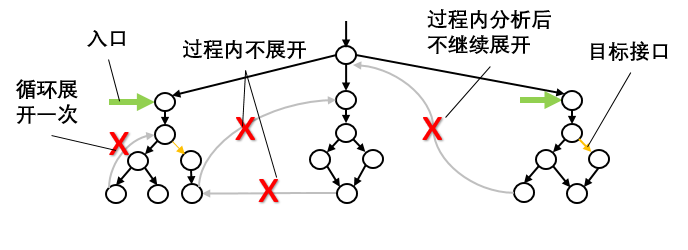
\includegraphics[width=0.9\linewidth]{figures/cp3-3-multi-entry.png}
	\caption{
		多入口分析策略示意图
	}
	\label{fig:3-3-multi-entry}
\end{figure}

\subsection{多入口分析策略}
经典的程序分析方法以主函数为入口,自顶向下对程序分析。
然而这种方式在面对大规模代码分析时,其分析效率存在巨大挑战。
因此,为支持大规模程序研究人员和分析工具开发人员选择逐函数的分析策略,
从而降低分析复杂度。
类似地,IMChecker采用多入口的分析策略,
即将一个复杂的程序分析问题分而治之,在保证全局有效规模化分析的同时,
尽可能提高局部分析精度。

如图\ref{fig:3-3-multi-entry}中示意图所示,
IMChecker在CFA上对目标接口的使用情况进行检索,
以包含目标接口$f$的函数调用上下文$c$作为分析入口。
如图中黄色边为$f$的调用指令,绿色箭头所指向的$c$为分析入口。
然而,基于函数入口进行分析,随着函数展开层数增加、循环展开,依旧面临着状态空间爆炸的问题。
因此,IMChecker在分析过程中,采取两个策略以支持大规模分析的同时,尽可能地降低精度损失:
\begin{itemize}
	\item 限制循环展开。
	循环展开问题是静态程序分析的难点之一。
	第\ref{sec:2.3}节的调研结果显示,绝大部分接口使用错误与循环无关。
	因此,IMChecker在分析的过程中,只展开一次循环以提高分析的效率。
	尽管这种策略会导致路径信息不全,降低分析的精度。但是,这并不会显著地影响分析的结果。
	\item 限制过程间分析。
	在IMChecker的分析过程中,通过符号执行的方式对每一个$c$进行路径提取。
	对函数展开会带来极大的分析负担,影响分析效率。
	同时,第\ref{sec:2.3}节的调研结果显示,大部分接口缺陷可以在过程内进行检测。
	所以,IMChecker在执行时对$c$内的其他函数调用不展开。
	同时在$c$执行后,不会继续执行。
	函数展开层数会影响接口使用缺陷检测的精度,本文将在过滤阶段通过引入上下文语义摘要信息过滤分析结果,
	以提高检测精度。
\end{itemize}


\subsection{抽象符号路径提取}
在缺陷检测之前,IMChecker通过符号执行(symbolic execution)对程序进行静态模拟执行,
并基于符号对程序路径的语义信息进行抽象描述。
该方法旨在保留接口相关的程序语义前提下尽可能简化程序结构。

\begin{figure}[t]
	\centering
	\footnotesize
		\begin{IEEEeqnarray*}{rCl}
			\text{(Traces) } \mathit{T} & ::= & \mathit{t} \\
			\text{(trace) } \mathit{t} & ::= & (id\_\mathit{a})^+; \mathit{V} \\
			\text{(action) } \mathit{a} & ::= & \text{\textbf{Assume}} (\mathit{exp}) ~|~ \text{\textbf{Call}} ~f(\mathit{sv}^*) ~|~ \text{\textbf{Return}} (\mathit{sv}) \\
			\text{(expression) } \mathit{exp} & ::= & \mathit{sv1}~\mathit{cmpop}~\mathit{sv2} \\
			\text{(value map) } V & ::= & \mathit{sv} \rightarrow \mathit{cv} \\
			\text{(symbolic variable) } \mathit{sv} & ::= & (id\_f\text{\textbf{\_arg\_}}\mathit{n}) \\
			\text{(compare operator) } cmpop & ::= & != ~|~ == ~|~ >= ~|~ > ~|~ <= ~|~ < \\
			\text{(concrete value) } \mathit{cv} & ::= & \mathit{z} ~|~ \mathit{ap} ~|~ \texttt{\textbf{NULL}}  \\
			\text{(function) } f & \in & \mathbb{F}
		\end{IEEEeqnarray*}	
	\caption{IMChecker路径信息提取抽象语法}
	\label{fig:3-3-path-syntax}
	
\end{figure}

令$\mathbb{N, Z}$表示非负整数和全体整数。
在图\ref{fig:3-3-path-syntax}中,本节给出IMChecker路径抽取的抽象语法结构。
其中,$id \in \mathbb{N}, n \in \mathbb{N}, z \in \mathbb{Z}$。
IMChecker关注整数和指针两种变量。
特别地,利用Accesspath~\cite{15-ase-accesspath}结构来代表内存地址,简写为$ap$。
$ap$的形式为正则语言$v(o|d)^*(o|\epsilon)$,
即$ap$是首地址$v$与偏移$o$和解引用$d$的组合。
每一条路径$\mathit{t}$由一系列的路径动作$\mathit{a}^+$和动作结束时值映射关系$\mathit{V}$组成。
需要说明的是,IMChecker基于LLVM-IR实现,所有的值只会被赋值一次,
所以只需要维护一个$\mathit{V}$即可。
IMChecker基于CFA图结构,在进行图遍历的时候进行动作提取和值分析。
因此,IMChecker支持流敏感(flow-sensitive)分析。
目前IMChecker关注三种程序语句:
if语句判断条件\textbf{Assume}、函数调用\textbf{Call}和返回值\textbf{Return}。
特别地,\textbf{Assume}能够有效地捕获路径可达性信息(path-sensitive)。
在分析过程中,IMChecker对每一个动作分配一个唯一的$id$,
以区别分析的上下文环境(context-sensitive)。
$\mathit{V}$记录符号变量$\mathit{sv}$到具体值$\mathit{cv}$的映射关系。
一个符号值由具体动作产生的$id$、产生的接口、以及对应的参数位置 $\mathit{n}$构成。
例如, $\mathit{id}\_f\_\textbf{arg}\_\mathit{i}$
表示第$id^{th}$动作为函数调用,其目标接口$f$的第$\mathit{i}^{th}$个参数。
特别地,IMChecker用0表示返回值索引,即$f\_\textbf{arg}\_0$表示接口$f$的返回值。
在\textbf{Return}中,用$\textbf{arg}\_0$表示$f$的调用者$c$的返回值。
%如果该符号值与函数、返回值无关,则直接通过$id$号来标识。
综上所示,IMChecker抽取的路径信息能够支持流敏感、路径敏感、上下文敏感的语义信息。

在图\ref{fig:3-3-path-example}中,给出图\ref{fig:1-1-example}代码片段的路径信息。
其中,“\_”为与例子不相关的变量。
图\ref{fig:1-1-example}代码片段共有三条路径,
$t_1$和$t_3$为原始代码的路径信息,$t_2$为修复后代码的路径信息。
所有三条路径起始于\texttt{X\_509\_get\_pubkey()}函数调用。
$t_1$直接将接口的返回值\textbf{1\_X509\_get\_pubkey\_arg\_0}传递给
\texttt{X509\_REQ\_set\_pubkey()},忽略对该返回值的检查。
$t_2$中,则对该返回值进行非空检测。
$t_3$中,同样没有直接对返回值进行检查,并直接传递给\texttt{check\_suite\_b()}的第一个参数。

\begin{figure}[t]
	\centering
	\footnotesize
		\begin{IEEEeqnarray*}{rCl}
			t_1:&~& \text{1\_\textbf{Call~} X509\_get\_pubkey(\_);}\\
			&~& \text{2\_\textbf{Call~} X509\_REQ\_set\_pubkey(\_, \textbf{1\_X509\_get\_pubkey\_arg\_0}) };\\
			t_2:&~& \text{1\_\textbf{Call~} X509\_get\_pubkey(\_);} \\
			&~& \text{2\_\textbf{Assume}(\textbf{1\_X509\_get\_pubkey\_arg\_0 != NULL}) }; \\
			&~& \text{3\_\textbf{Call~} X509\_REQ\_set\_pubkey(\_, \textbf{1\_X509\_get\_pubkey\_arg\_0}) }; \\
			t_3:&~& \text{1\_\textbf{Call~} X509\_get\_pubkey(\_);} \\
			&~& \text{2\_\textbf{Call~} check\_suite\_b(\textbf{1\_X509\_get\_pubkey\_arg\_0}, \_, \_) ;}
		\end{IEEEeqnarray*}	
	\caption{图~\ref{fig:1-1-example}中抽象路径提取结果}
	\label{fig:3-3-path-example}
\end{figure}
%~& \text{2\_\textbf{Assume}(\textbf{1_X509_get_pubkey_arg_0 != NULL}) }; &

\subsection{缺陷检测算法}

\IncMargin{1em}
\begin{algorithm}[t]
	\SetAlgorithmName{算法}{heuristic}{IMSpec分解算法}
	\SetKwData{Spec}{Spec}
	\SetKwData{spec}{spec}
	\SetKwData{Map}{SpecMap}
	\SetKwData{item}{item}
	\SetKwData{Continue}{continue}
	\SetKwData{TraceMap}{Trace\_{Map}}
	\SetKwData{CFA}{CFA}
	\SetKwFunction{Union}{Union}
	\SetKwFunction{CheckIPU}{SatisfyIPU}
	\SetKwFunction{CheckIEH}{SatisfyIEH}
	\SetKwFunction{CheckICC}{SatisfyICC}
	\SetKwFunction{Extract}{Extract}
	\SetKwFunction{New}{NewItem}
	\SetKwInOut{Input}{输入}\SetKwInOut{Output}{输出}
	
	\Input{分解后的规约集合 \Map,符号路径轨迹映射\TraceMap}
	\Output{缺陷报告 ${R}$}
	\BlankLine
	\For{\Map 中的每个实例 \item}{
		$R \leftarrow \emptyset$\;
		$T \leftarrow$ \Extract(\item.target)\;
		\For{$T$ 中的每一条路径 $t$}{
			\If{\item.IPU 存在}{
				\ForEach{\item.IPU中的$p$}{
					$b$ $\leftarrow$ \CheckIPU($p$, $t$)\;
					\lIf{$!b$}{
						$R$ $\leftarrow$ \Union(\item.target, $R$, $p$, $t$)
					}
				}
			}
			\If{\item.IEH 存在}{
				\ForEach{\item.IEH中的$eh$}{
					$b$ $\leftarrow$ \CheckIEH($pt$, $t$)\;
					\lIf{$!b$}{
						$R$ $\leftarrow$ \Union(\item.target, $R$, $eh$, $t$)
					}
				}
			}
			\If{\item.ICC 存在}{
				\ForEach{\item.IEH中的$cc$}{
					$b$ $\leftarrow$ \CheckICC($cc$, $t$)\;
					\lIf{$!b$}{
						$R$ $\leftarrow$ \Union(\item.target, $R$, $cc$, $t$)
					}
				}
			}
		}
	}
	\caption{IMChecker缺陷检测算法}
	\label{alg:cp3-3-detect}
\end{algorithm}\DecMargin{1em}
IMChecker的缺陷检测算法如算法\ref{alg:cp3-3-detect}中所示,
以分解后的SpecMap和符号路径轨迹映射Trace\_Map作为输入,以缺陷检测结果$R$为输出。
其中,符号路径轨迹映射是接口到包含该接口路径集合$T$:
$$\text{Trace\_Map}: f \rightarrow T$$
缺陷检测结果,是目标接口到缺陷信息(违反的约束$s_{item}$和路径$t$)的集合:
$$R: f \rightarrow (s_{item}, t)$$
IMChecker对每一个约束实例item中的目标接口进行相关路径提取获得路径集合$T$,
再对集合中的每一条独立的子路径$t$进行分析。
路径分析包含三个部分,分别对应于约束的三个模式,即IPU、IEH和ICC。

SatisfyIPU对使用约束中的前置条件进行检测:
(1)如果在路径$t$中存在语义等价的\textbf{Assume},
那么该约束$p$则满足;反之如果\textbf{Assume}与$p$的语义相反,那么该路径则一定错误。
(2)如果在路径$t$中不存在语义等价的\textbf{Assume},
那么则在路径上对目标接口的函数调用动作\textbf{Call}中的值映射关系$V$中判断$p$是否满足。
如果满足则为路径对目标接口使用正确,反之不正确。

SatisfyIEH对使用约束中后置条件中异常处理相关的约束进行检测。
每一个$eh=(cond, a^+)$由两部分组成,
错误路径发生条件$cond$
(即$cond$是包含目标接口的返回值$ret$的布尔表达式,表示该情况下目标接口发生错误)
和异常处理动作$a^+$(即异常处理路径上需要进行的异常处理操作)。
因此,在缺陷检测时首先判断路径是否为缺陷发生路径,再判断异常处理动作是否满足约束:
(1)在目标函数调用后的子轨迹$t'$中,判断是否存在\textbf{Assume}动作,
该动作与$ret$相关。如果不存在,则路径缺少了错误代码检查,为错误使用。
在相关的\textbf{Assume}动作中,如果\textbf{Assume}与$cond$不等价则为非异常处理路径,不需要继续分析。
(2)在异常处理路径上,对$a^+$中的每个约束进行判断,是否存在等价的路径动作。
其中,函数调用约束对应于\textbf{Call}动作分析,返回值约束对应于\textbf{Return}动作分析。
如果存在不满足的约束,那么这条轨迹为错误使用。

SatisfyICC对使用约束中后置条件中因果调用关系相关的约束进行检测。
每一个$cc=(cond, g)$由两部分组成,
因果调用关系上下文语义约束$cond$(即只有在$cond$满足的情况下才调用后续接口),
和因果调用关系的第二个接口$g$。
因此,在缺陷检测时分为两种情况:
(1)
$cond$为True(即目标接口和$g$不存在上下文约束关系),那么如果不存在等价于$g$的\textbf{Call}动作,路径为错误使用。
(2)
$cond$不为True。
一方面,如果存在\textbf{Assume}动作等价于$cond$,则需要对$g$进行检查。
其中,如果不存在等价的\textbf{Call},路径为误用;
反之为正确使用。
另一方面,如果存在\textbf{Assume}动作不等价于$cond$,则判断是否存在与$g$等价的\textbf{Call}。
如果存在等价的\textbf{Call}动作,那么路径使用错误。

本文以图\ref{fig:3-3-path-example}中的路径作为例子进行解释。
接口\texttt{X509\_get\_pubkey()}用于解码证书,当发生错误时其返回NULL作为错误代码。
所以,其返回值需要进行检查,即IMSpec规约为
\begin{lstlisting}[language={[ANSI]C},
basicstyle=\linespread{0.8}\listingsfont,
numbers=none,
xleftmargin=.15\textwidth]
(*@\textcolor{blue}{Target:}@*) X509_get_pubkey(_) -> _
(*@\textcolor{blue}{Post:}@*) 
	// 需要对错误状态代码进行检查,检查的约束为返回值不是NULL
	- X509_get_pubkey_arg_0 != NULL
\end{lstlisting}
然而在图\ref{fig:3-3-path-example}中,只有路径$t_2$进行显式地检测,
即存在路径动作
\begin{lstlisting}[language={[ANSI]C},
basicstyle=\linespread{0.8}\listingsfont,
numbers=none,
xleftmargin=.15\textwidth]
2_Assume(1_X509_get_pubkey_arg_0 != NULL)
\end{lstlisting}
因此,IMChecker认为路径$t_1, t_3$为错误使用路径,
被加入到缺陷报告$R$中。

\subsection{检测结果过滤}
为支持规模化接口缺陷检测,IMChecker采用多入口分析策略,并在分析过程中对函数展开和循环展开进行限制。
这种分析策略会忽略跨越函数的上下文语义信息,损失静态分析的精度,导致大量的误报。
例如图\ref{fig:3-3-path-example}中的例子,
虽然$t_1, t_3$都缺少必要的返回值检测,然而如图\ref{fig:1-1-example}中代码27行所示,
\begin{lstlisting}[language={[ANSI]C},
basicstyle=\linespread{0.7}\listingsfont,
numbers=none,
xleftmargin=.25\textwidth]
(*@\textcolor{mauve}{pk = X509\_get\_pubkey(x);}@*)
rv = check_suite_b((*@\textcolor{mauve}{pk}@*), -1, &tflags);
	
static int check_suite_b(EVP_PKEY *(*@\textcolor{mauve}{pkey}@*),...){
	[(*@\dots@*)]
	// ensure pkey not NULL
	(*@\textcolor{mauve}{if (pkey \&\& ...)}@*)
\end{lstlisting}
轨迹$t_3$在参数使用的位置确保该指针不为空,即$t_3$为误报。
为解决上述精度损失问题,IMChecker通过两种策略对结果进行过滤,以提升检测精度。

\paragraph{跨函数语义摘要}
跨函数的语义摘要过滤方式,旨在通过对跨函数的语义信息计算对检测结果进行过滤。
通过对实际项目的预实验后,IMChecker目前对四种情况进行过滤。
令$f$为目标接口,$r$为$f$的返回值且携带错误状态信息,$c$为调用$f$的函数,
$g$为需要同$f$协同使用的因果调用函数,$H$为$c$中除$f$的函数调用集合。
则过滤的模式为:
\begin{itemize}
	\item $r$赋值给$c$的参数。一种常见的情况为,$f$为资源申请函数(例如\texttt{malloc}),
	并将申请后的指针$r$赋值给$c$(\texttt{foo})的参数(ptr),
	并在$c$的上下文中对$r$进行管理。例如下列代码片段,
	\begin{lstlisting}[language={[ANSI]C},
	basicstyle=\linespread{0.7}\listingsfont,
	numbers=none,
	xleftmargin=.15\textwidth]
	int foo(char **ptr) {
		*ptr = (char *)malloc(100*sizeof(char));
		return 1;
	}
	int bar(){
		char *p = NULL;
		foo(&p);
		// handle p
	}
	\end{lstlisting}
	因此,在$c$的函数体内,并没有对该指针检查或者释放。
	\item $r$赋值给$c$的返回值。与上述情况相似,$c$直接返回$r$,
	例如下列代码片段,
		\begin{lstlisting}[language={[ANSI]C},
	basicstyle=\linespread{0.7}\listingsfont,
	numbers=none,
	xleftmargin=.15\textwidth]
	char *foo(int size) {
		char *data;
		data = (char *)malloc(size*sizeof(char));
		return data;	
	}
	int bar(){
		char *p = NULL;
		p = foo(100);
		// handle p
	}
	\end{lstlisting}
	\item $r$作为$h \in H$的参数使用。
	一种常见的API使用方式是在接口的实现内进行参数检测。
	因此,如果$r$作为参数传递给$h$,并且$h$对参数检查,那么$f$的使用则正确。
	例图\ref{fig:1-1-example}例子中$t_3$的情况。
	\item $g$在将$r$作为参数的$h \in H$中调用,即$r$约束满足,$f-g$需要协同使用(\texttt{malloc/free})。
	在$c$中(\texttt{foo}),$r$(data)满足约束,并作为$h$(\texttt{bar})的参数,而且$g$在$h$中调用。
	例如下列代码,
			\begin{lstlisting}[language={[ANSI]C},
	basicstyle=\linespread{0.7}\listingsfont,
	numbers=none,
	xleftmargin=.15\textwidth]
	
	void bar(char *p) {
		if (p != NULL) free(p);
	}
	void foo(){
		char * data = (char *)malloc(100*sizeof(char));
		if (data == NULL) return;
		bar(data);
	    ...
	}
	\end{lstlisting}
	
\end{itemize}

\paragraph{接口误用统计信息}
实际项目中的接口使用情况多种多样、部分接口具有特殊用法、用户提供错误的IMSpec等等都会导致检测工具产生误报。
为过滤这些误报提升检测精度并对结果进行有效排序,
IMChecker通过基于使用情况的统计信息进行结果优化。
在分析过程中,IMChecker分别计算正确使用路径$u_T$和错误路径$u_F$的个数。
首先,对于所有使用次数$u_T+u_F$小于最小支持度$\alpha$(minimum support)的目标接口$f$的缺陷报告,
IMChecker归纳为低置信度(confidence)。
IMChecker将该缺陷归纳为警告(Warning)。
例如,一个目标接口只有一次使用并不符合用户提供的约束,很难判断检测结果的正确性。
对于超过$\alpha$的目标接口,
IMChecker根据错误置信度$\mathcal{H}$,
\begin{equation}
\label{eq:3-1}
\mathcal{H}  = ({u_T-u_F})\times\dfrac{u_T}{u_F}
\end{equation}
对结果进行排序。
当正确使用与错误使用的比例越大时,则认为越多的正确使用强烈地支持这个误用为错误。
当比例相同时,认为正确的次数比错误的次数多时,则可信度更高。
例如,$\mathcal{H}(u_T=2, u_F=1)$与$H(u_T=3, u_F=2)$相比,前者的比例更高;
$H(u_T=3, u_F=1)$与$H(u_T=6, u_F=2)$相比,则后者更可信。
特别地,当$\mathcal{H} \le 1$时,即错误与正确一样多或者多于正确使用时,
IMChecker将该缺陷归纳为警告类型。

\section{工具实现与实验评估}
\label{sec:3.4}
本节首先介绍规模化接口误用缺陷检测方法IMChecker的实现细节。
随后在公开数据集上,对IMChecker的分析能力进行评估,并给出IMChecker与主流开源工具的比较结果。

\begin{figure}[t]
	\centering
	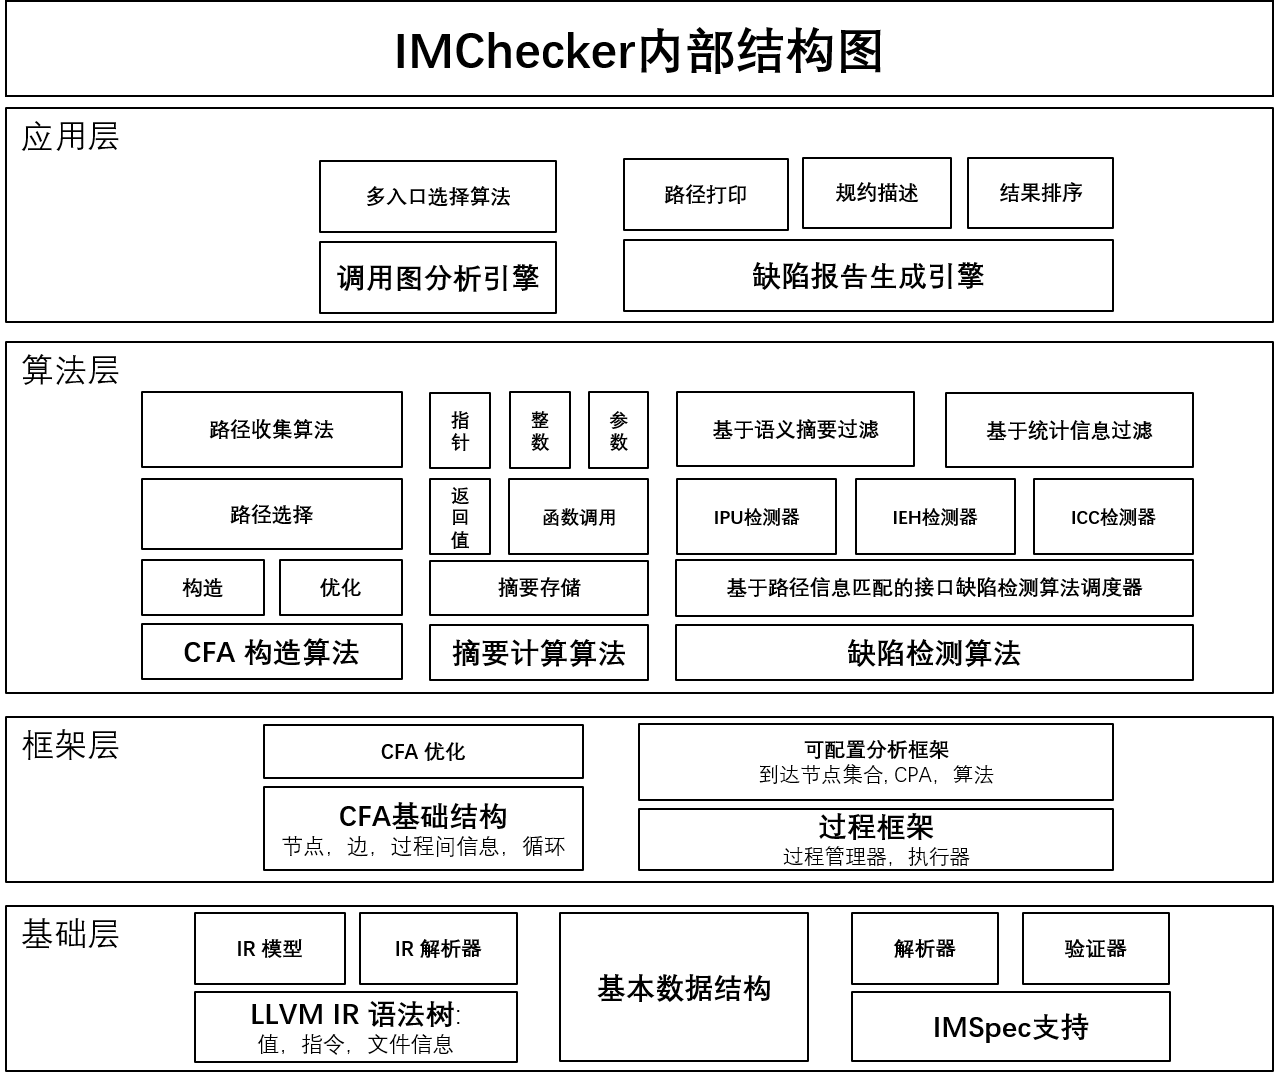
\includegraphics[width=0.9\linewidth]{figures/cp3-implementation.png}
	\caption{
		IMChecker工具实现内部结构图
	}
	\label{fig:3-4-implementation}
\end{figure}

\subsection{工具实现}
IMChecker基于Java语言实现,依赖LLVM3.9的IR作为中间表达,
并基于CPA~\cite{07-cav-cpachecker}算法作为整体方法的实现基础。
工具以用户提供的源代码和IMSpec规约描述作为输入。
其中IMSpec实例和缺陷检测结果都基于Yaml~\cite{yaml}格式存储。
工具实现的内部结构如图\ref{fig:3-4-implementation}所示,
共包含四个层次:基础层、架构层、算法层和应用层。
首先,基础层通过对源代码进行预处理,生成LLVM-IR中间表达;
并对IMSpec规约描述进行解析、一致性分析和规约化简。
框架层构造CFA,将程序转化为图结构;
同时,提供CPA算法的分析流程以支持上层语义计算。
算法层,则对CFA进行优化、计算语义摘要信息以及缺陷检测。
最后,应用层通过函数调用图具体进行分析入口的选择,执行缺陷分析;
并将缺陷检测的结果进行过滤、排序和信息打印。

\paragraph{基础层}
基础层旨在对用户输入的源代码和IMSpec规约描述进行预处理,同时提供分析中需要的基本数据结构。
首先,对于用户输入的源代码,
如果待测程序是单个的C文件,IMChecker直接使用clang编译器
\begin{lstlisting}[language={bash},
basicstyle=\linespread{0.8}\listingsfont,
numbers=none,
xleftmargin=.25\textwidth]
(*@\textcolor{blue}{Ubuntu@~: clang}@*) path2source -S -emit-llvm -g
\end{lstlisting}
进行预处理以生成自包含的*.ll文件。
该文件相比于*.c源文件增加必需的函数和数据结构声明、展开宏定义、消除预处理指令等,
并生成对应的LLVM-IR中间表达。
如果待测程序是一个Makefile工程,
那么通过解析Makefile中的编译指令并且将所有输出*.o文件的指令替换为相应的预处理指令,例如clang -E。
通过预处理生成的*.i文件,利用上述指令生成*.ll文件。
同时,根据Makefile的编译目标将项目组织成不同的分析任务。
通过llvm的链接指令(llvm-link)将给定分析任务下所有的*.ll文件进行合并,
作为输入进行缺陷检测。
在获得LLVM-IR中间表达后,利用javacpp\footnote{https://github.com/bytedeco/javacpp}工具解析文件,
并构造IR模型,包括值、指令和文件信息。
另一方面,基础层对用户提供的IMSpec语言进行解析。
IMSpec语言面向单个目标接口设计,所以如果规约中存在语法错误则将错误规约忽略并输出给使用者。
同时,解析后的IMSpec进行语义一致性验证,即是否存在冲突的约束。
例如,一个条件是接口的第一个参数大于零,另一个条件是第一个参数小于零等等。

\paragraph{框架层}
框架层旨在提供分析框架的实现以及CFA基础结构的创建。
在对用户提供的源代码解析过后,CFA基础结构模块对LLVM-IR进行包装,创建CFA图结构。
特别地,CFA在节点上表示程序的位置,在边上封装程序的具体执行指令。
为在CFA图上提供更多的语义信息,
本文将CFA边分为两种,即控制边和摘要边。
前者表示具体的语义操作的指令,例如存储、运算、返回等等。
后者表示函数调用和循环关系。
因此,通过摘要边在分析中可以利用摘要信息跳过函数展开和循环遍历,
从而保证大规模代码有效分析的同时提高分析精度。
IMChecker基于过程(Phase)来运行,即每个过程负责不同的预处理或者检测步骤。
所以,框架层中实现过程管理的调度器。
特别地,IMChecker基于CPA算法来实现具体的路径抽取和缺陷检测。
因此IMChecker在框架层实现CPA算法的核心数据结构和基础调度算法,
具体的每一个CPA则在算法层中实现。

\paragraph{算法层}
算法层旨在实现具体的算法细节。
IMChecker针对C程序接口误用缺陷进行检测,具体的实现可以分为三个模块:
路径收集、摘要计算和缺陷检测。
\begin{itemize}
	\item {\kaishu 路径收集} 
	在路径收集阶段,IMChecker利用CFA构造算法,对框架层的CFA原型进行优化。
	特别地,为支持大规模程序分析,IMChecker基于入口分析。
	因此,在这个阶段对入口进行标记。
	此后,基于优化后的CFA图结构,通过第\ref{sec:3.3}节中的路径抽取方法,
	收集路径信息,为后续两个步骤做准备。
	目前IMChecker基于AccessPath~\cite{15-ase-accesspath}和整数分析对语义信息进行计算。
	\item {\kaishu 摘要计算} 
	摘要计算的结果将被应用于缺陷检测当中。
	在实现层面,IMChecker则先进行摘要的计算。
	为支持大规模程序检测,IMChecker采用基于多入口分析的策略,使得跨函数语义信息丢失分析精度下降,
	导致误报。
	为提供更加准确的检测结果,IMCHecker利用上下文语义信息对结果进行过滤。
	具体而言,IMChecker计算:上下文指针常量计算、整数常量计算、参数约束关系、
	返回值常量关系和函数调用关系的摘要信息。
	\item {\kaishu 缺陷检测} 
	缺陷检测部分,IMChecker实现基于路径信息匹配的接口误用缺陷检测算法。
	特别地,为提高检测精度IMChecker实现检测算法调度器,
	即根据使用约束的不同调用不同的检测算法实现,以精确分析程序进行缺陷检测。
	最后,利用基于语义的摘要信息和基于使用情况的统计信息对结果过滤。
\end{itemize}


\paragraph{应用层}
应用层旨在从工具实际运行的角度,对IMChecker进行封装和优化。
一方面,应用层实现多入口选择算法和调度引擎。
通过该模块,具体执行每个入口的分析。
另一方面,对于检测后的缺陷,生成相应的缺陷报告,
包括:缺陷产生的路径信息、违反的约束和IMSpec与自然语言两种形式的解释信息。
特别地,IMChecker基于使用情况对缺陷检测结果进行排序。

IMChecker已经集成在Tsmart工具集中~\cite{tsmart},工具使用的具体细节将在第\ref{sec:4.3}节中进行介绍。

\subsection{实验准备}



\paragraph{测试集} 
由于目前并没有针对C程序接口误用缺陷检测的测试集合,
因此本文基于美国国家标准技术研究所(NIST) 整理的Juliet Test Suite测试集~\cite{juliet},
对IMChecker的分析能力进行评估。
该测试集合包含超过6万个C/C++用例,涵盖118个不同的CWE缺陷类型,
是目前最为广泛使用的测试集。
本文根据接口误用缺陷模式共选取13个具体的分类。
Juliet测试集合在每个分类中给出大量重复模式、不同产生原因的测试用例。
因此,本文对其中重复的用例进行过滤,保留由于接口误用导致错误的测试用例。
同时,对每个分类中的缺陷实例进行过滤和修正,
以确保每个测试用例至少含有一个误用和一个修复后的版本。
如表\ref{tab:3-4-cwe}所示,针对第\ref{sec:2.3}节中总结的三大类接口误用模式,
本文共选取2172个测试用例。
为方便研究人员和开发者理解缺陷模式和评估检测工具,
本文将这些修订后的测试用例集成到C程序接口误用缺陷数据集APIMU4C中,
并公开在Github中\footnote{https://github.com/imchecker/compsac19/tree/master/APIMU4C}。

\begin{table}[t]
	\centering
	\begin{minipage}[t]{0.8\linewidth} % 如果想在表格中使用脚注,minipage是个不错的办法
		\caption{评估测试集组成}
		\label{tab:3-4-cwe}
		\begin{tabular}{cccl}
			\hline
			{缺陷类别 } & {CWEID} & 缺陷数目 & \multicolumn{1}{c}{缺陷描述} \\
			\hline
			\multirow{6}{*}{IPU} & 121 & 36 & 栈内存越界读取\\
			& 122 & 36 & 堆内存越界读取 \\
			& 131 & 42 & 不正确的计算缓冲区大小\\
			& 476 & 36 & 空指针引用\\
			& 590 & 360 & 释放非堆内存\\
			\cline{2-4} 
			& \multicolumn{3}{c}{5个CWE分类,510个测试用例} \\
			\hline
			\multirow{3}{*}{IEH} & 252 & 270 & 未检查错误状态代码\\
			& 253 & 270 & 错误状态代码检查不正确\\
			& 390 & 72 & 未进行异常处理\\
			\cline{2-4} 
			& \multicolumn{3}{c}{3个CWE分类,612个测试用例} \\
			\hline
			\multirow{5}{*}{ICC} & 401 & 474 & 内存泄漏\\
			& 404 & 24 & 不正确的资源释放\\
			& 415 & 120 & 重复释放\\
			& 690 & 384 & 未对因果调用中的上下文关系检测\\
			& 775 & 48 & 未释放文件资源\\
			\cline{2-4} 
			& \multicolumn{3}{c}{5个CWE分类,1050个测试用例} \\
			\hline
		\end{tabular}
	\end{minipage}
\end{table}
\paragraph{比较对象}
首先,为检测过滤机制的效果,本文将未添加过滤机制的方法记作为IMChecker--。
通过IMChecker与IMChecker--在测试集上的分析结果评估过滤算法的有效性。
此外,本文选取广泛使用的代表性开源工具进行检测能力的比较。
在对工具描述文档阅读、学术论文研究和工具预实验后,本文共选取如下三个工具:
\begin{itemize}
	\item APISan~\cite{16-sec-apisan}(主分支-2018-0601):
	该工具是一个开源的学术工具,针对接口误用缺陷设计。
	通过数据挖掘技术与程序分析技术结合,利用轻量级语义分析方法获得接口使用上下文信息,
	并基于统计方法推理接口使用约束。
	工具基于过程内分析方法,考虑函数返回值、参数关系和因果调用关系,并将规约推理的结果用于缺陷检测。
	不过,推理出的中间结果(接口使用的约束)没有输出,也没有提供扩展规约推理方法或者接收约束的接口。
	\item Cppcheck~\cite{cppcheck}(版本1.83):
	Cppcheck是针对未定义和危险程序结构的缺陷检测工具。
	该工具开源代码,并支持多个领域和不同的缺陷类型。
	将代码转化为字节流(token)后,
	基于上下文敏感(context-sensitive)和流敏感(flow-sensitive)的过程间分析方法,
	对缺陷进行模式匹配。
	Cppcheck在检测算法中集成C标准库的接口。
	同时,为支持用户自定义的接口,
	提供一套规约描述方法\footnote{http://cppcheck.sourceforge.net/manual.pdf, chapter10, page 20.},
	以利用实现过的算法对相同的缺陷模式进行检测。
	例如参数空指针,内存泄漏等等。
	\item Clang-SA~\cite{clang-sa}(版本RELEASE\_600):
	该工具是LLVM开源编译器的组成部分。
	通过符号执行技术,推理程序语义。
	该工具采用上下文敏感(context-sensitive)和流敏感(flow-sensitive)的过程间分析方法,
	并实现大量的检测插件,以应对不同的缺陷类型\footnote{http://clang-analyzer.llvm.org/available checks.html}。
	该工具可以通过开发新的检测插件从而支持用户自定义的接口。
	然而,需要理解内部数据结构表达和分析流程,开发难度较大。
\end{itemize} 
一方面,这三个工具提供良好的缺陷报告接口,支持多种接口缺陷类型。
另一方面,这三个工具基于不同的分析技术(数据挖掘、静态分析-硬编码、静态分析-基于规约描述)。
同时,三个工具在预实验中的检测能力稳定,与文档论文中的描述能力一致。

\paragraph{评测指标}
在测试集上,本文将采用如下两个指标对工具进行评估:
\begin{itemize}
	\item 召回率(Recall):$R = \dfrac{\text{结果报告中真实的缺陷数}}{\text{总缺陷数}}$。
	召回率是基于具体实现情况下,工具的检测能力,即工具能够有效地检测多少缺陷。
	缺陷检测领域普遍认为,一个工具在测试集合上的召回率越高,那么其实际应用中也会有更好的检测效果。
	\item 精度(Precision):$P = \dfrac{\text{结果报告中真实的缺陷数}}{\text{工具报告的缺陷总数}}$。
	研究表明,阻碍实际用户使用静态分析工具的原因之一是现有工具产生大量的误报,即精度太低~\cite{10-acm-precision}。
	因此,检测工具的精度是重要的指标之一。
	%特别地,如果精度低于30\%,那么实际使用者将抛弃这个工具。
\end{itemize}
%\item 理想召回率(Conceptual Recall,CR):$= \dfrac{理想情况下能够支持的缺陷数}{工具报告的缺陷总数}$
%该指标表示工具能够支持的最大程序的检测能力。即,工具用户手册或者论文中,不考虑实现的正确性下,提到能够解决问题的全部空间。一个工具的CR越高,代表这个工具的检测能力越强。 $R = \frac{结果报告中真实的缺陷数}{总缺陷数}$

\paragraph{运行环境} 本文在一台装有64位Ubuntu 16.04的台式机上进行实验,
该机器配有Intel(R) Core(R) i5-3470@3.20GHz-4核心CPU和32GB内存。
本章关注接口缺陷检测的能力,因此不设置最长分析时间。


\subsection{评测结果}

\begin{table}[b]
	\centering
	\begin{minipage}[t]{0.9\linewidth} % 如果想在表格中使用脚注,minipage是个不错的办法
		\caption{IMChecker评测结果}
		\label{tab:3-4-imchecker}
		\begin{tabular}{cccccccccc}
			\hline
			\multirow{2}{*}{类别 } & \multirow{2}{*}{个数} & \multicolumn{4}{c}{IMChecker} & \multicolumn{4}{c}{IMChecker-~-} \\
			\cline{3-10}
			 & & 报告数 & TP\footnote{TP:真实缺陷数目} & P(\%) & R(\%) & 报告数 & TP& P(\%) & R(\%) \\
			 \hline
			 IPU & 510 & 490 & 423 & 86.33 & 82.94 & 745 & 469 & 62.95 & 91.96 \\
			 IEH & 612 & 580 & 506 & 87.24 & 82.68 & 677 & 526 & 77.70 & 85.94 \\
			 ICC & 1050 & 1012 & 878 & 86.76 & 83.62 & 1320 & 898 & 68.03 & 85.52 \\
			 总计 & 2172 &  2082 & 1807 & 86.79 & 83.20 & 2742 & 1893 & 69.04 & 87.15 \\
			\hline
		\end{tabular}
	\end{minipage}
\end{table}
\paragraph{IMChecker评测结果}
评测结果如表\ref{tab:3-4-imchecker}中所示,
其中报告数为工具缺陷的总报告数,TP为报告中真实存在的缺陷数目,P为精度,R为召回率。
表中3-6列为IMChecker的评估结果,7-10列为IMChecker--的评测结果(即不包括过滤机制的结果)。

评测结果表明,在所有的测试用例中,
IMChecker--共产生2742个缺陷报告,其中1893个为真实缺陷,
849个误报,平均精度为69.04\%,平均召回率为87.15\%。
在对缺陷报告深入分析后,导致IMChecker--分析结果不准确的主要原因是跨函数的接口使用。
如第\ref{sec:3.3}节中所示,为能够支持大规模代码有效分析,IMChecker的检测算法基于过程内分析进行。
因此,当接口使用跨函数时,则会导致分析精度下降。

本文通过\texttt{malloc/free}例子进行分析。
在C的标准库中,两者组合进行堆内存的申请和释放。
其使用约束是,当前者的返回值不为NULL时,需要调用后者进行释放。
然而IMChecker--基于过程内的分析方式,对于跨越函数调用的接口,分析精度不足。
一方面,语义信息的不足会产生误报,即将正确的用法报告为缺陷。
例如下面代码所示,
\begin{lstlisting}[language={C},
basicstyle=\linespread{0.7}\listingsfont,
numbers=left,
xleftmargin=.3\textwidth]
void bar(int* p){
	// do
	free(p);
}
void foo(){
	int* p = (int*) malloc(100*sizeof(int));
	if (p == NULL) return;
	bar(p);
}
\end{lstlisting}
IMChecker--在第6行发现调用\texttt{malloc}函数,在第7行对返回值进行检测,
需要调用\texttt{free}函数进行内存释放。
然而该释放操作在第3行的\texttt{bar}函数内进行,
因此IMChecker--并没有捕获这样的信息,导致将该用例判断为缺陷,产生一个误报。
另一方面,同样的语义信息不足则可能导致漏报,即没有检测到缺陷。
\begin{lstlisting}[language={C},
basicstyle=\linespread{0.7}\listingsfont,
numbers=left,
xleftmargin=.3\textwidth]
void bar(int* p){
	// do
	free(p);
}
void foo(){
	int* p = (int*) malloc(100*sizeof(int));
	if (p == NULL) return;
	bar(p);
	free(p);
}
\end{lstlisting}
例如上述代码所示,IMChecker--在第9行检测到\texttt{free}函数。
同时该函数的参数与\texttt{malloc}的返回值指向同一块内存。
因此,IMChecker--会将该用例判断为缺陷。
然而,在\texttt{bar}函数内,已经对该指针所指向的内存释放。
所以这是一个重复释放内存错误(CWE-590)。

因此,需要消除跨函数语义带来的影响,解决上述问题以提高检测的精度。
如第\ref{sec:3.3}节介绍,IMChecker引入基于语义和基于使用情况的过滤机制。
在结合过滤算法后,IMChecker共产生2082个缺陷报告,其中1807个为真实缺陷。
IMChecker的平均精度为86.79\%,平均召回率为83.20\%。
相比较于IMChecker--,在有限的召回率损失下(3.95\%),
IMChecker检测精度有显著提高(17.75\%)。
损失的召回率由于过滤机制中,对于参数和返回值的处理造成。
%\begin{lstlisting}[language={C},
%basicstyle=\linespread{0.7}\listingsfont,
%numbers=left,
%xleftmargin=.2\textwidth]
%void foo(int **p) {
%	*p = (int*) malloc(100*sizeof(int));
%	// do
%}
%\end{lstlisting}
在实际项目中,本文发现大量的内存申请结果赋值给参数或者返回值并在外界进行检测和维护。
因此,IMChecker将这种情况下的缺陷过滤能够有效减少误报。
然而如果外界缺少必要的操作,则会产生漏报。
同时,虽然引入过滤机制,IMChecker依旧存在误报和漏报。
目前,IMChecker基于语义的过滤机制只关注一层函数调用的摘要信息。
因此,当调用信息超过两层时,依旧无法准确检测。
例如如下代码片段,
\begin{lstlisting}[language={C},
basicstyle=\linespread{0.7}\listingsfont,
numbers=left,
xleftmargin=.35\textwidth]
void bar2(int* p){        
	// do						   
	free(p);					  
}
void bar1(int* p){        
	// do						   
	bar2(p);					  
}
void foo(){...}
\end{lstlisting}
由于释放函数跨越两层调用,因此无法被过滤,IMChecker将产生一个误报。


此外其他一些原因同样导致IMChecker分析不够精确,包括:
\begin{itemize}
	\item 复杂的数据依赖关系。
	目前IMChecker基于CPA算法实现,通过AccessPath的方式记录指向关系,并维护整数信息。
	然而,当指针存在偏移操作时,如果偏移的位置不为常量,那么IMChecker就会认为这个指针指向该内存对象所有的区间。
	另一方面,由于目前只维护常量整数,当整数为变量时,IMChecker会认为该值可能为任何值。
	例如,\texttt{memcpy(d,s,n)}拷贝内存内容,
	拷贝的长度n应小于目标d的大小。
	然而当程序中,无法对n和d的关系进行推理时,IMChecker则会认为是错误,从而产生误报。
	\item 函数指针。
	C程序提供函数指针的语言特性。然而在静态分析阶段,无法明确获取该指针的指向关系。
	IMChecker在分析的过程中会忽略这部分内容,导致误报和漏报。
	\item 循环。
	循环问题在程序分析中是至今无法良好解决的难题。
	特别地,如第\ref{sec:3.3}节缺陷实例调研结果显示,
	接口误用缺陷很少发生在循环中。
	因此,IMChecker只展开一次循环。
	对于如下代码中的重复释放问题,IMChecker则会产生漏报。
\begin{lstlisting}[language={C},
basicstyle=\linespread{0.7}\listingsfont,
numbers=left,
xleftmargin=.2\textwidth]
	char * data;
	data = NULL;
	for(i = 0; i < 1; i++){
		data = (char *)malloc(100*sizeof(char));
		strcpy(data, "A String");
	}
	for(k = 0; k < 2; k++){
		free(data);
	}
\end{lstlisting}	
\end{itemize}

针对于上述总结的不足,一个可行的解决方案是引入更加精确的分析方法。
例如,增加跨函数分析、增加循环展开、增加函数指针的映射关系、利用更精确的值分析方法等等。
然而这些精确的语义计算会极大地影响分析效率。
因此,如何平衡分析效率与精度需要更多的尝试。
本文将在第\ref{cha:con}章中进行描述。

\paragraph{IMChecker与其他工具对比结果}

\begin{table}[b]
	\centering
	\begin{minipage}[t]{0.9\linewidth} % 如果想在表格中使用脚注,minipage是个不错的办法
		\caption{对比工具评测结果}
		\label{tab:3-4-other}
		\begin{tabular}{cccccccccc}
			\hline
			\multirow{2}{*}{类别 } & \multirow{2}{*}{个数} & \multicolumn{2}{c}{APISan} & \multicolumn{2}{c}{Cppcheck} & \multicolumn{2}{c}{Clang-SA} & \multicolumn{2}{c}{IMChecker}\\
			\cline{3-10}
			 & & 报告数 & TP & 报告数 & TP& 报告数 & TP & 报告数 & TP \\
			 \hline
			 IPU & 510 &  154 & 48 & 145 &127 &127 &105 & 490 & 423\\
			 IEH & 612 &  446 &173& 298& 270& 0& 0& 580& 506 \\
			 ICC & 1050 &  447 &435 &373 &337 &746& 565 &1012 &878 \\
			 总计 & 2172 &   1047& 656& 816& 734& 873& 670& 2082& 1807 \\
			 \multicolumn{2}{c}{平均-P\%} &\multicolumn{2}{c}{62.66}  & \multicolumn{2}{c}{89.95}  &\multicolumn{2}{c}{76.75}  &\multicolumn{2}{c}{86.79} \\
			 \multicolumn{2}{c}{平均-R\%} & \multicolumn{2}{c}{30.20} & \multicolumn{2}{c}{33.79}  &\multicolumn{2}{c}{30.85}  &\multicolumn{2}{c}{83.20}  \\
			\hline
		\end{tabular}
	\end{minipage}
\end{table}

表\ref{tab:3-4-other}中对四个工具的评测结果进行总结。
其中Cppcheck的检测精度最高,达到89.95\%,
其次是IMChecker为86.79\%和Clang-SA为76.75\%,
APISan的准确率最低,为62.66\%。
在检测能力方面,IMChecker的召回率最高,为83.20\%,
其他三个工具的检测能力则相对较低,在30-35\%之间。

{\kaishu{基于推理方式的APISan}} 通过推理的方式学习接口使用的约束,
并根据语义的差异性对缺陷进行检测。
与基于数据挖掘技术的检测方法一致,
工具的检测能力由预先定义的缺陷模式决定。
APISan工具封装$A \rightarrow B$的使用约束,
即A调用后需要调用B接口。
然而,并没有对$A \rightarrow \neg B$模式进行定义。
因此该工具忽略所有的重复释放(double free)用例,
占ICC分类的11.43\%。
此外,APISan的学习结果无法保存和跨项目使用。
因此,只能针对于单个测试用例或者项目进行分析。
当缺少足够的数据对接口使用约束条件进行学习时,
APISan将无法获得正确的使用约束。
这导致APISan无法支持11.11\%的缺陷用例。
另一方面,基于挖掘技术的方法多基于程序的语法形式分析,
无法支持隐含的语义信息。
例如,APISan能够学习显式的语义信息,包括条件语句中的条件判断、函数调用等等。
然而,无法推理出隐式的语义约束。
例如,不包含显式检查的内存读写接口中参数的关系。
另外,有一些语义信息无法通过C的语法进行描述,则必然会被忽略。
例如,释放非堆内存错误,
程序需要对\texttt{free}的参数所指向的内存区域进行深入的语义分析。

{\kaishu {基于程序分析方式的Clang-SA和Cppcheck}}工具将接口使用约束编码在独立的检测插件中,
在程序分析的过程中,对缺陷直接检测。
Clang-SA提供各种针对于不同缺陷类型的检测插件。
例如,security.insecureAPI.UncheckedReturn插件用来检测忽略对函数返回值检测的接口误用缺陷。
然而,并没有一个插件能够支持测试用例中IEH缺陷,
导致Clang-SA漏报所有IEH的缺陷实例。

项目特定的接口经常会和C标准库中的接口具有相同的使用约束。
例如,用户自定义的\texttt{*\_new}接口,与\texttt{malloc}行为一致,
对资源进行管理。
在资源生命周期结束后,需要进行释放操作。
没有提供可扩展的静态分析工具则无法对这类接口进行分析。
因此,Clang-SA难以支持所有的缺陷用例。
Cppcheck提供面向特定项目的规约描述方法,以支持用户自定义的接口。
然而,该语言的描述能力不足,检测能力提升有限。
例如,Cppcheck只支持对常量的返回值进行定义,
且不能够描述形如$a - [cond] - b$带有上下文语义约束的函数调用。

本文从表\ref{tab:3-4-other}中发现,相对于高检测精度,
Clang-SA和Cppcheck的召回率非常低。
在对两个工具的原理和测试结果分析后,
本文发现两个工具采取一种保守策略,
即为提高检测精度增加工具的友好性,只对具有高可能性的缺陷进行报告。
因此,相同的缺陷模式在复杂的代码结构中将会被忽视。

\noindent\textbf{总结:}对于三个比较的工具,在深入分析实验结果后本文发现,
与IMChecker相比这些工具对语义分析不足,导致大量的漏报。
具体体现在:
(1)缺少路径敏感度分析(path-sensitive)。
对路径的可达性分析在静态分析中具有重要意义。
例如,在\texttt{malloc}内存申请成功后,当某条异常处理路径上没有释放内存时,
将会产生一个内存泄漏错误。
然而,当申请失败时,则不需要释放。
因此,分析需要对路径信息进行维护和记录,而不是简单的通过调用次数进行缺陷检测。
(2)缺少过程间分析(inter-procedural)。
当接口使用跨越函数调用时,需要基于过程间信息来进行程序分析。
例如,\texttt{malloc/free}在两个函数中。


综上所述,在测试集上IMChecker取得86.79\%的检测精度和83.20\%的召回率。
检测能力优于比较的三个知名工具。
其中,相比较于Clang-SA和APISan,具有更高的检测精度和检测能力。
在精度基本一致的情况下(86.79\%与89.95\%),比Cppcheck多检测(49.41\%)的缺陷。


\section{本章小结}
\label{sec:3.5}
本章提出基于约束描述的规模化C程序接口误用缺陷检测方法IMChecker。
IMChecker利用IMSpec语言对接口使用约束进行描述,以支持用户自己定义的接口以及多种缺陷模式。
同时,IMChecker采用多入口分析策略,将复杂的程序分析问题分而治之,
高效率分析的同时实现局部的精确分析。
对于多入口分析策略引入的精度损失而导致的误报,
IMChecker通过基于上下文语义的摘要信息和基于使用情况的统计信息对结果进行过滤,以提高检测精度。
在Juliet Test Suite公开测试集上13个接口缺陷相关分类的评测结果显示,
IMChecker方法误报率为13.21\%,漏报率为16.08\%,
检测能力领先于主流的开源软件项目。
